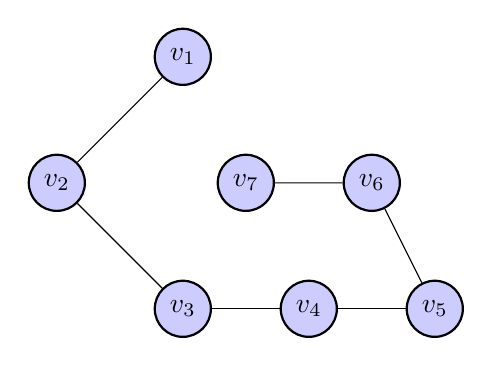
\begin{tikzpicture}
  [scale=.8,auto=left,every node/.style={circle,fill=blue!20,draw=black,thick}]
  \node (n1) at (2,4) {$v_1$};
  \node (n2) at (0,2)  {$v_2$};
  \node (n3) at (2,0)  {$v_3$};
  \node (n4) at (4,0) {$v_4$};
  \node (n5) at (6,0)  {$v_5$};
  \node (n6) at (5,2)  {$v_6$};
  \node (n7) at (3,2)  {$v_7$};

  \foreach \from/\to in {n1/n2,n2/n3, n3/n4, n4/n5, n5/n6, n6/n7}
    \draw (\from) -- (\to);
\end{tikzpicture}
